\documentclass[border=5pt]{standalone}
\usepackage[dvipsnames]{xcolor}
\usepackage{tikz}
\usetikzlibrary{arrows.meta,positioning,calc,fit}
\usepackage{amssymb}

\definecolor{cL0}{HTML}{9E9E9E}
\definecolor{cL1}{HTML}{1E88E5}
\definecolor{cL2}{HTML}{F9A825}
\definecolor{cL3}{HTML}{8E24AA}
\definecolor{cL4}{HTML}{D32F2F}
\definecolor{cChain}{HTML}{E65100}
\definecolor{cTTP}{HTML}{00897B}
\definecolor{cProto}{HTML}{37474F}

\begin{document}
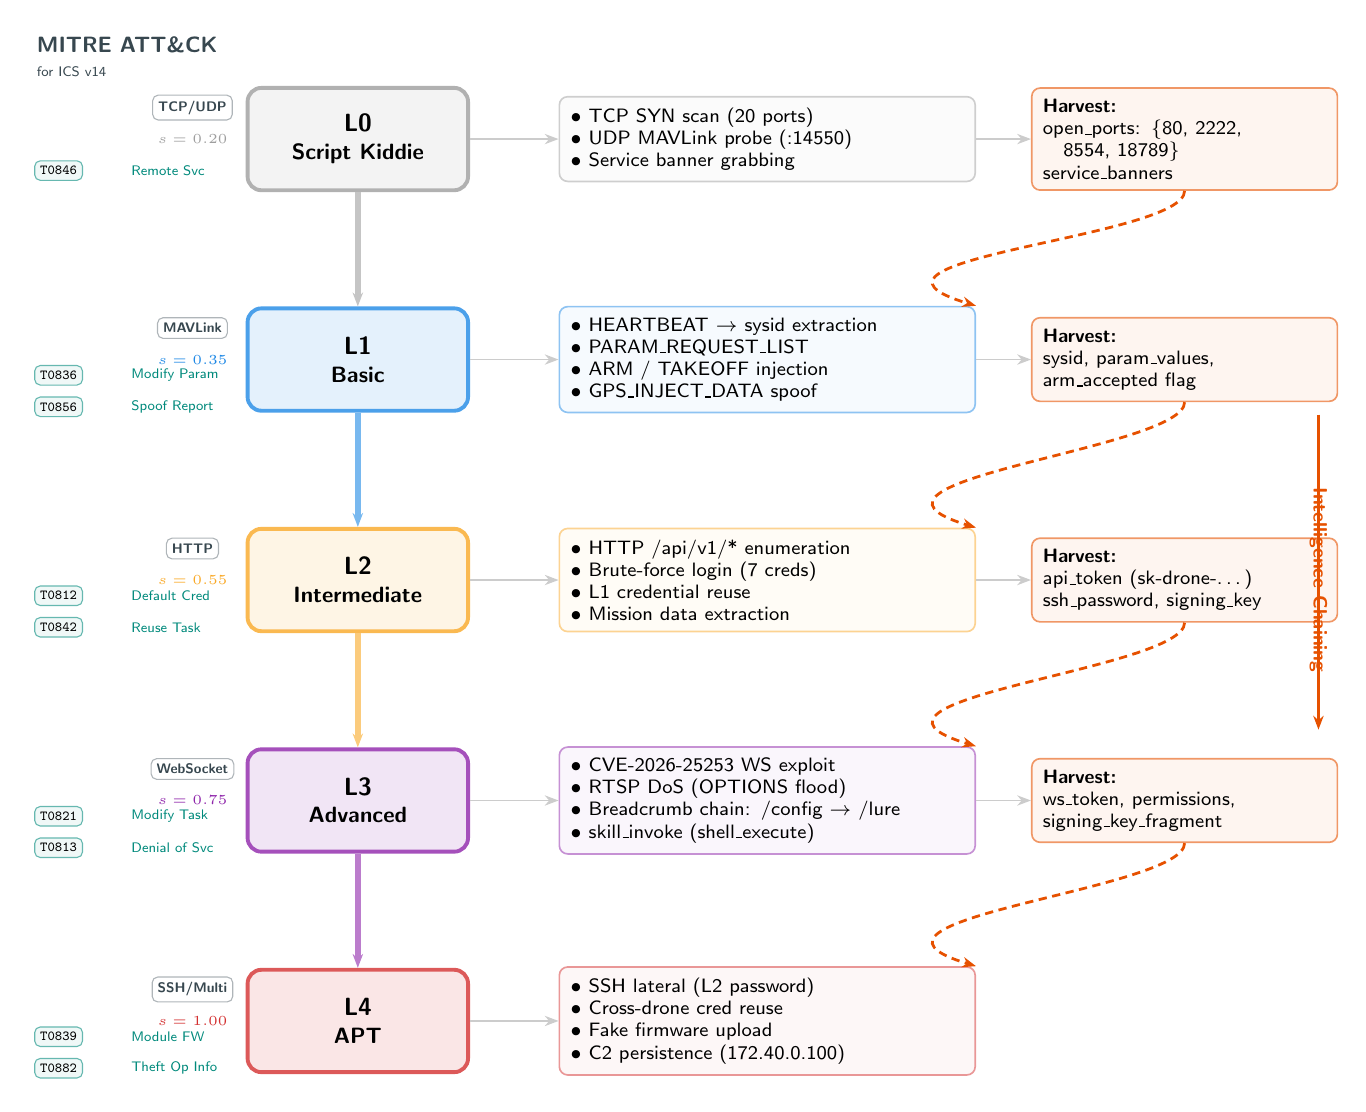
\begin{tikzpicture}[
  >={Stealth[length=5pt]},
  font=\sffamily,
  lvl/.style={
    rectangle, rounded corners=5pt, draw=#1!80, fill=#1!12,
    line width=1.4pt, minimum width=2.8cm, minimum height=1.3cm,
    align=center, font=\sffamily\bfseries\small
  },
  action/.style={
    rectangle, rounded corners=3pt, draw=#1!50, fill=#1!4,
    line width=0.6pt, align=left, font=\sffamily\scriptsize,
    text width=5.0cm, inner sep=4pt
  },
  harvest/.style={
    rectangle, rounded corners=3pt, draw=cChain!60, fill=cChain!6,
    line width=0.6pt, align=left, font=\sffamily\scriptsize,
    text width=3.6cm, inner sep=4pt
  },
  ttp/.style={
    rectangle, rounded corners=2pt, draw=cTTP!60, fill=cTTP!6,
    font=\ttfamily\tiny, inner sep=2pt
  },
  proto/.style={
    rectangle, rounded corners=2pt, draw=cProto!40, fill=white,
    font=\sffamily\tiny\bfseries, inner sep=2pt, text=cProto
  },
  cascade/.style={->, line width=2pt, draw=#1!60},
  chain/.style={->, line width=1pt, draw=cChain, densely dashed},
  link/.style={->, line width=0.5pt, draw=gray!40},
]

% Vertical spacing
\def\dy{-2.8}

% ════════════════════════════════════════════════════
% Level nodes (left column)
% ════════════════════════════════════════════════════
\node[lvl=cL0] (L0) at (0, 0*\dy) {L0\\[-1pt]{\footnotesize Script Kiddie}};
\node[lvl=cL1] (L1) at (0, 1*\dy) {L1\\[-1pt]{\footnotesize Basic}};
\node[lvl=cL2] (L2) at (0, 2*\dy) {L2\\[-1pt]{\footnotesize Intermediate}};
\node[lvl=cL3] (L3) at (0, 3*\dy) {L3\\[-1pt]{\footnotesize Advanced}};
\node[lvl=cL4] (L4) at (0, 4*\dy) {L4\\[-1pt]{\footnotesize APT}};

% ── Cascade arrows ──────────────────────────────────
\draw[cascade=cL0] (L0) -- (L1);
\draw[cascade=cL1] (L1) -- (L2);
\draw[cascade=cL2] (L2) -- (L3);
\draw[cascade=cL3] (L3) -- (L4);

% ── Skill param s ───────────────────────────────────
\node[font=\sffamily\tiny, text=cL0] at (-2.1, 0*\dy) {$s=0.20$};
\node[font=\sffamily\tiny, text=cL1] at (-2.1, 1*\dy) {$s=0.35$};
\node[font=\sffamily\tiny, text=cL2] at (-2.1, 2*\dy) {$s=0.55$};
\node[font=\sffamily\tiny, text=cL3] at (-2.1, 3*\dy) {$s=0.75$};
\node[font=\sffamily\tiny, text=cL4] at (-2.1, 4*\dy) {$s=1.00$};

% ── Protocol labels ─────────────────────────────────
\node[proto] at (-2.1, 0*\dy+0.4) {TCP/UDP};
\node[proto] at (-2.1, 1*\dy+0.4) {MAVLink};
\node[proto] at (-2.1, 2*\dy+0.4) {HTTP};
\node[proto] at (-2.1, 3*\dy+0.4) {WebSocket};
\node[proto] at (-2.1, 4*\dy+0.4) {SSH/Multi};

% ════════════════════════════════════════════════════
% Action boxes (center column)
% ════════════════════════════════════════════════════
\node[action=cL0] (A0) at (5.2, 0*\dy) {
  $\bullet$ TCP SYN scan (20 ports)\\
  $\bullet$ UDP MAVLink probe (:14550)\\
  $\bullet$ Service banner grabbing
};
\node[action=cL1] (A1) at (5.2, 1*\dy) {
  $\bullet$ HEARTBEAT $\to$ sysid extraction\\
  $\bullet$ PARAM\_REQUEST\_LIST\\
  $\bullet$ ARM / TAKEOFF injection\\
  $\bullet$ GPS\_INJECT\_DATA spoof
};
\node[action=cL2] (A2) at (5.2, 2*\dy) {
  $\bullet$ HTTP /api/v1/* enumeration\\
  $\bullet$ Brute-force login (7 creds)\\
  $\bullet$ L1 credential reuse\\
  $\bullet$ Mission data extraction
};
\node[action=cL3] (A3) at (5.2, 3*\dy) {
  $\bullet$ CVE-2026-25253 WS exploit\\
  $\bullet$ RTSP DoS (OPTIONS flood)\\
  $\bullet$ Breadcrumb chain: /config $\to$ /lure\\
  $\bullet$ skill\_invoke (shell\_execute)
};
\node[action=cL4] (A4) at (5.2, 4*\dy) {
  $\bullet$ SSH lateral (L2 password)\\
  $\bullet$ Cross-drone cred reuse\\
  $\bullet$ Fake firmware upload\\
  $\bullet$ C2 persistence (172.40.0.100)
};

\draw[link] (L0.east) -- (A0.west);
\draw[link] (L1.east) -- (A1.west);
\draw[link] (L2.east) -- (A2.west);
\draw[link] (L3.east) -- (A3.west);
\draw[link] (L4.east) -- (A4.west);

% ════════════════════════════════════════════════════
% Harvest boxes (right column)
% ════════════════════════════════════════════════════
\node[harvest] (H0) at (10.5, 0*\dy) {
  \textbf{Harvest:}\\
  open\_ports: \{80, 2222,\\
  \quad 8554, 18789\}\\
  service\_banners
};
\node[harvest] (H1) at (10.5, 1*\dy) {
  \textbf{Harvest:}\\
  sysid, param\_values,\\
  arm\_accepted flag
};
\node[harvest] (H2) at (10.5, 2*\dy) {
  \textbf{Harvest:}\\
  api\_token (sk-drone-\ldots)\\
  ssh\_password, signing\_key
};
\node[harvest] (H3) at (10.5, 3*\dy) {
  \textbf{Harvest:}\\
  ws\_token, permissions,\\
  signing\_key\_fragment
};

\draw[link] (A0.east) -- (H0.west);
\draw[link] (A1.east) -- (H1.west);
\draw[link] (A2.east) -- (H2.west);
\draw[link] (A3.east) -- (H3.west);

% ════════════════════════════════════════════════════
% Intelligence Chaining (diagonal orange dashed)
% ════════════════════════════════════════════════════
\draw[chain] (H0.south) .. controls +(0,-0.6) and +(-2,0.6) .. (A1.north east);
\draw[chain] (H1.south) .. controls +(0,-0.6) and +(-2,0.6) .. (A2.north east);
\draw[chain] (H2.south) .. controls +(0,-0.6) and +(-2,0.6) .. (A3.north east);
\draw[chain] (H3.south) .. controls +(0,-0.6) and +(-2,0.6) .. (A4.north east);

% Chain label
\node[rotate=-90, font=\sffamily\scriptsize\bfseries, text=cChain] at (12.2, -5.6) {Intelligence Chaining};
\draw[cChain, line width=0.8pt, ->] (12.2,-3.5) -- (12.2,-7.5);

% ════════════════════════════════════════════════════
% ATT&CK TTP tags (far left)
% ════════════════════════════════════════════════════
\node[ttp] (T0) at (-3.8, 0*\dy-0.4) {T0846};
\node[font=\sffamily\tiny, text=cTTP, anchor=west] at (-3.0, 0*\dy-0.4) {Remote Svc};

\node[ttp] (T1a) at (-3.8, 1*\dy-0.2) {T0836};
\node[font=\sffamily\tiny, text=cTTP, anchor=west] at (-3.0, 1*\dy-0.2) {Modify Param};
\node[ttp] (T1b) at (-3.8, 1*\dy-0.6) {T0856};
\node[font=\sffamily\tiny, text=cTTP, anchor=west] at (-3.0, 1*\dy-0.6) {Spoof Report};

\node[ttp] (T2a) at (-3.8, 2*\dy-0.2) {T0812};
\node[font=\sffamily\tiny, text=cTTP, anchor=west] at (-3.0, 2*\dy-0.2) {Default Cred};
\node[ttp] (T2b) at (-3.8, 2*\dy-0.6) {T0842};
\node[font=\sffamily\tiny, text=cTTP, anchor=west] at (-3.0, 2*\dy-0.6) {Reuse Task};

\node[ttp] (T3a) at (-3.8, 3*\dy-0.2) {T0821};
\node[font=\sffamily\tiny, text=cTTP, anchor=west] at (-3.0, 3*\dy-0.2) {Modify Task};
\node[ttp] (T3b) at (-3.8, 3*\dy-0.6) {T0813};
\node[font=\sffamily\tiny, text=cTTP, anchor=west] at (-3.0, 3*\dy-0.6) {Denial of Svc};

\node[ttp] (T4a) at (-3.8, 4*\dy-0.2) {T0839};
\node[font=\sffamily\tiny, text=cTTP, anchor=west] at (-3.0, 4*\dy-0.2) {Module FW};
\node[ttp] (T4b) at (-3.8, 4*\dy-0.6) {T0882};
\node[font=\sffamily\tiny, text=cTTP, anchor=west] at (-3.0, 4*\dy-0.6) {Theft Op Info};

% ── Title ───────────────────────────────────────────
\node[font=\sffamily\bfseries\footnotesize, text=cProto, anchor=west] at (-4.2, 1.2)
  {MITRE ATT\&CK};
\node[font=\sffamily\tiny, text=cProto, anchor=west] at (-4.2, 0.85) {for ICS v14};

\end{tikzpicture}
\end{document}
